\begin{figure}[tp]
  \centering
  \begin{tikzpicture}
    \node (si-label) at (0.0\textwidth, 0.16\textwidth) [] {Spaceship Indoor};
    \node (pa-label) at (0.3\textwidth, 0.16\textwidth) [] {Piper's Alley};
    \node (zc-label) at (0.6\textwidth, 0.16\textwidth) [] {Ziggurat City};

    \node[rotate=90] at (-0.16\textwidth - 15pt, -0.6\textwidth) {Knoopgrootte}; 
    \node[rotate=90] at (-0.16\textwidth,  0.0\textwidth) {0.25};
    \node[rotate=90] at (-0.16\textwidth, -0.3\textwidth) {0.5};
    \node[rotate=90] at (-0.16\textwidth, -0.6\textwidth) {1};
    \node[rotate=90] at (-0.16\textwidth, -0.9\textwidth) {2};
    \node[rotate=90] at (-0.16\textwidth, -1.2\textwidth) {3};

    \node[inner sep=0pt] (img1) at (0.0\textwidth, 0.0\textwidth) {
\includegraphics[width=0.275\textwidth]{./img/raw/hs-ns-frames-render/spaceship-indoor/0.png}};
    \node[inner sep=0pt] (img1) at (0.0\textwidth,-0.28\textwidth) {
\includegraphics[width=0.275\textwidth]{./img/raw/hs-ns-frames-render/spaceship-indoor/1.png}};
    \node[inner sep=0pt] (img1) at (0.0\textwidth,-0.56\textwidth) {
\includegraphics[width=0.275\textwidth]{./img/raw/hs-ns-frames-render/spaceship-indoor/2.png}};
    \node[inner sep=0pt] (img1) at (0.0\textwidth,-0.84\textwidth) {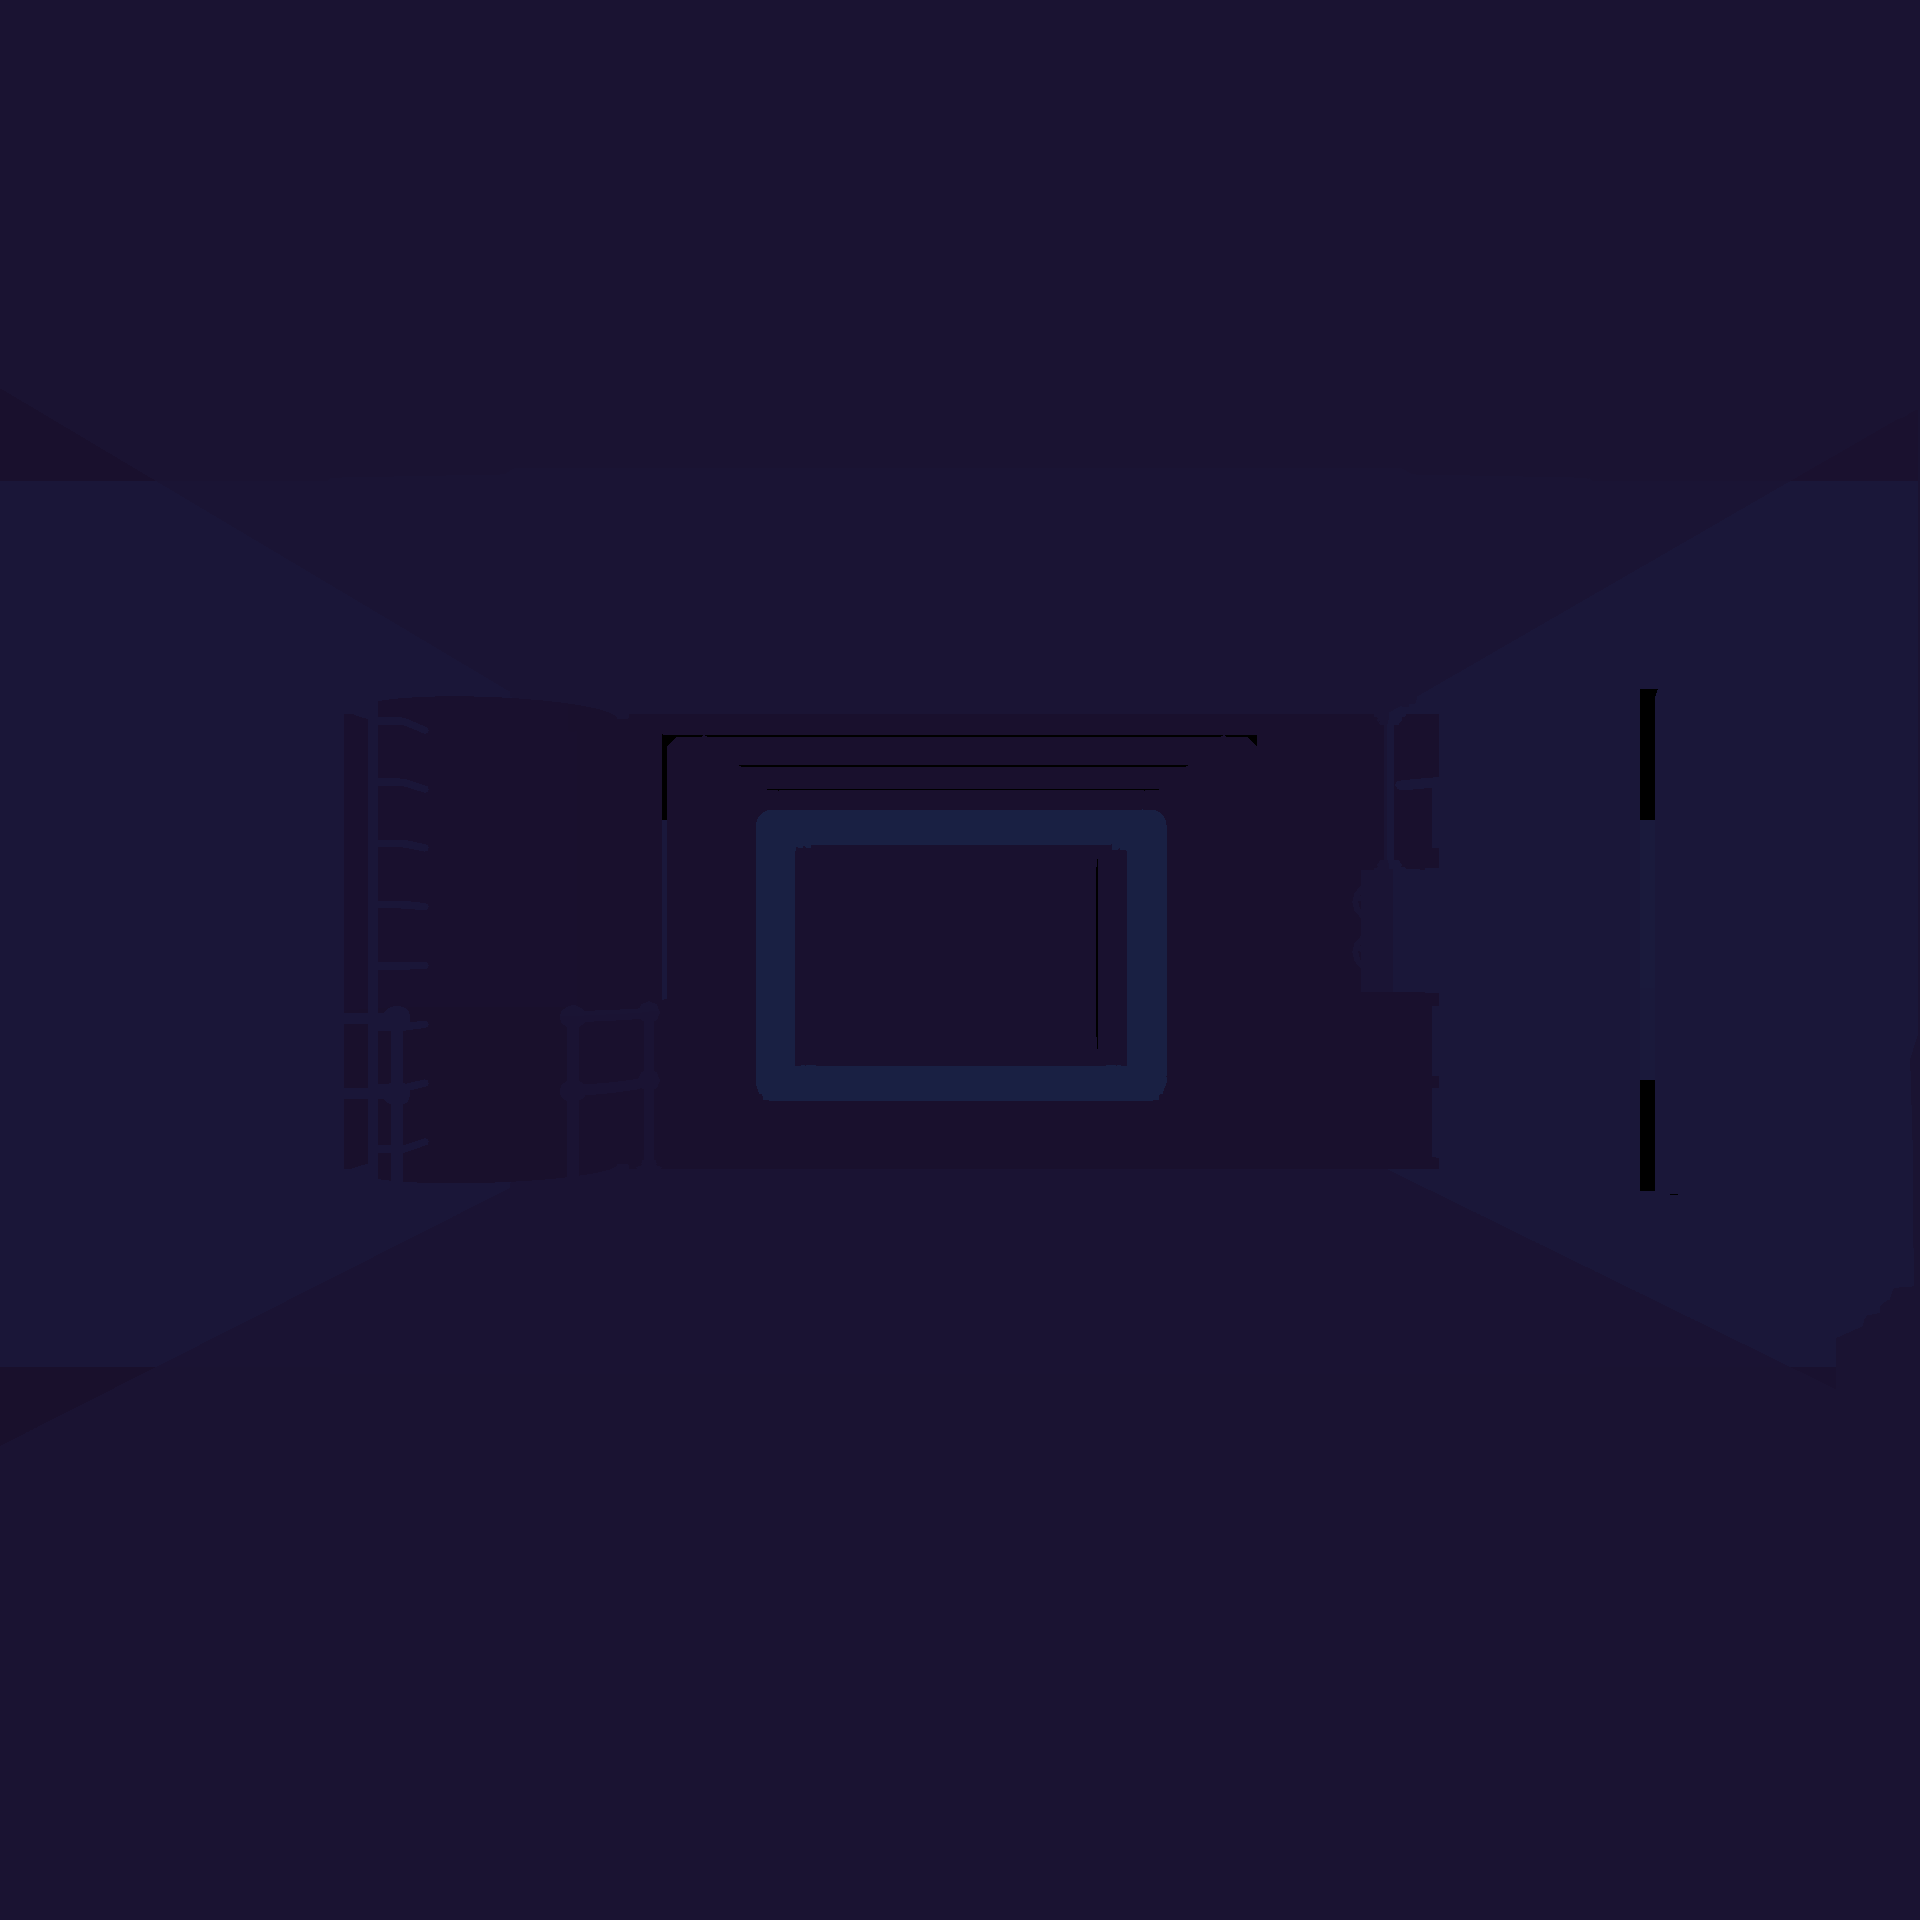
\includegraphics[width=0.275\textwidth]{./img/raw/hs-ns-frames-render/spaceship-indoor/3.png}};
    \node[inner sep=0pt] (img1) at (0.0\textwidth,-1.12\textwidth) {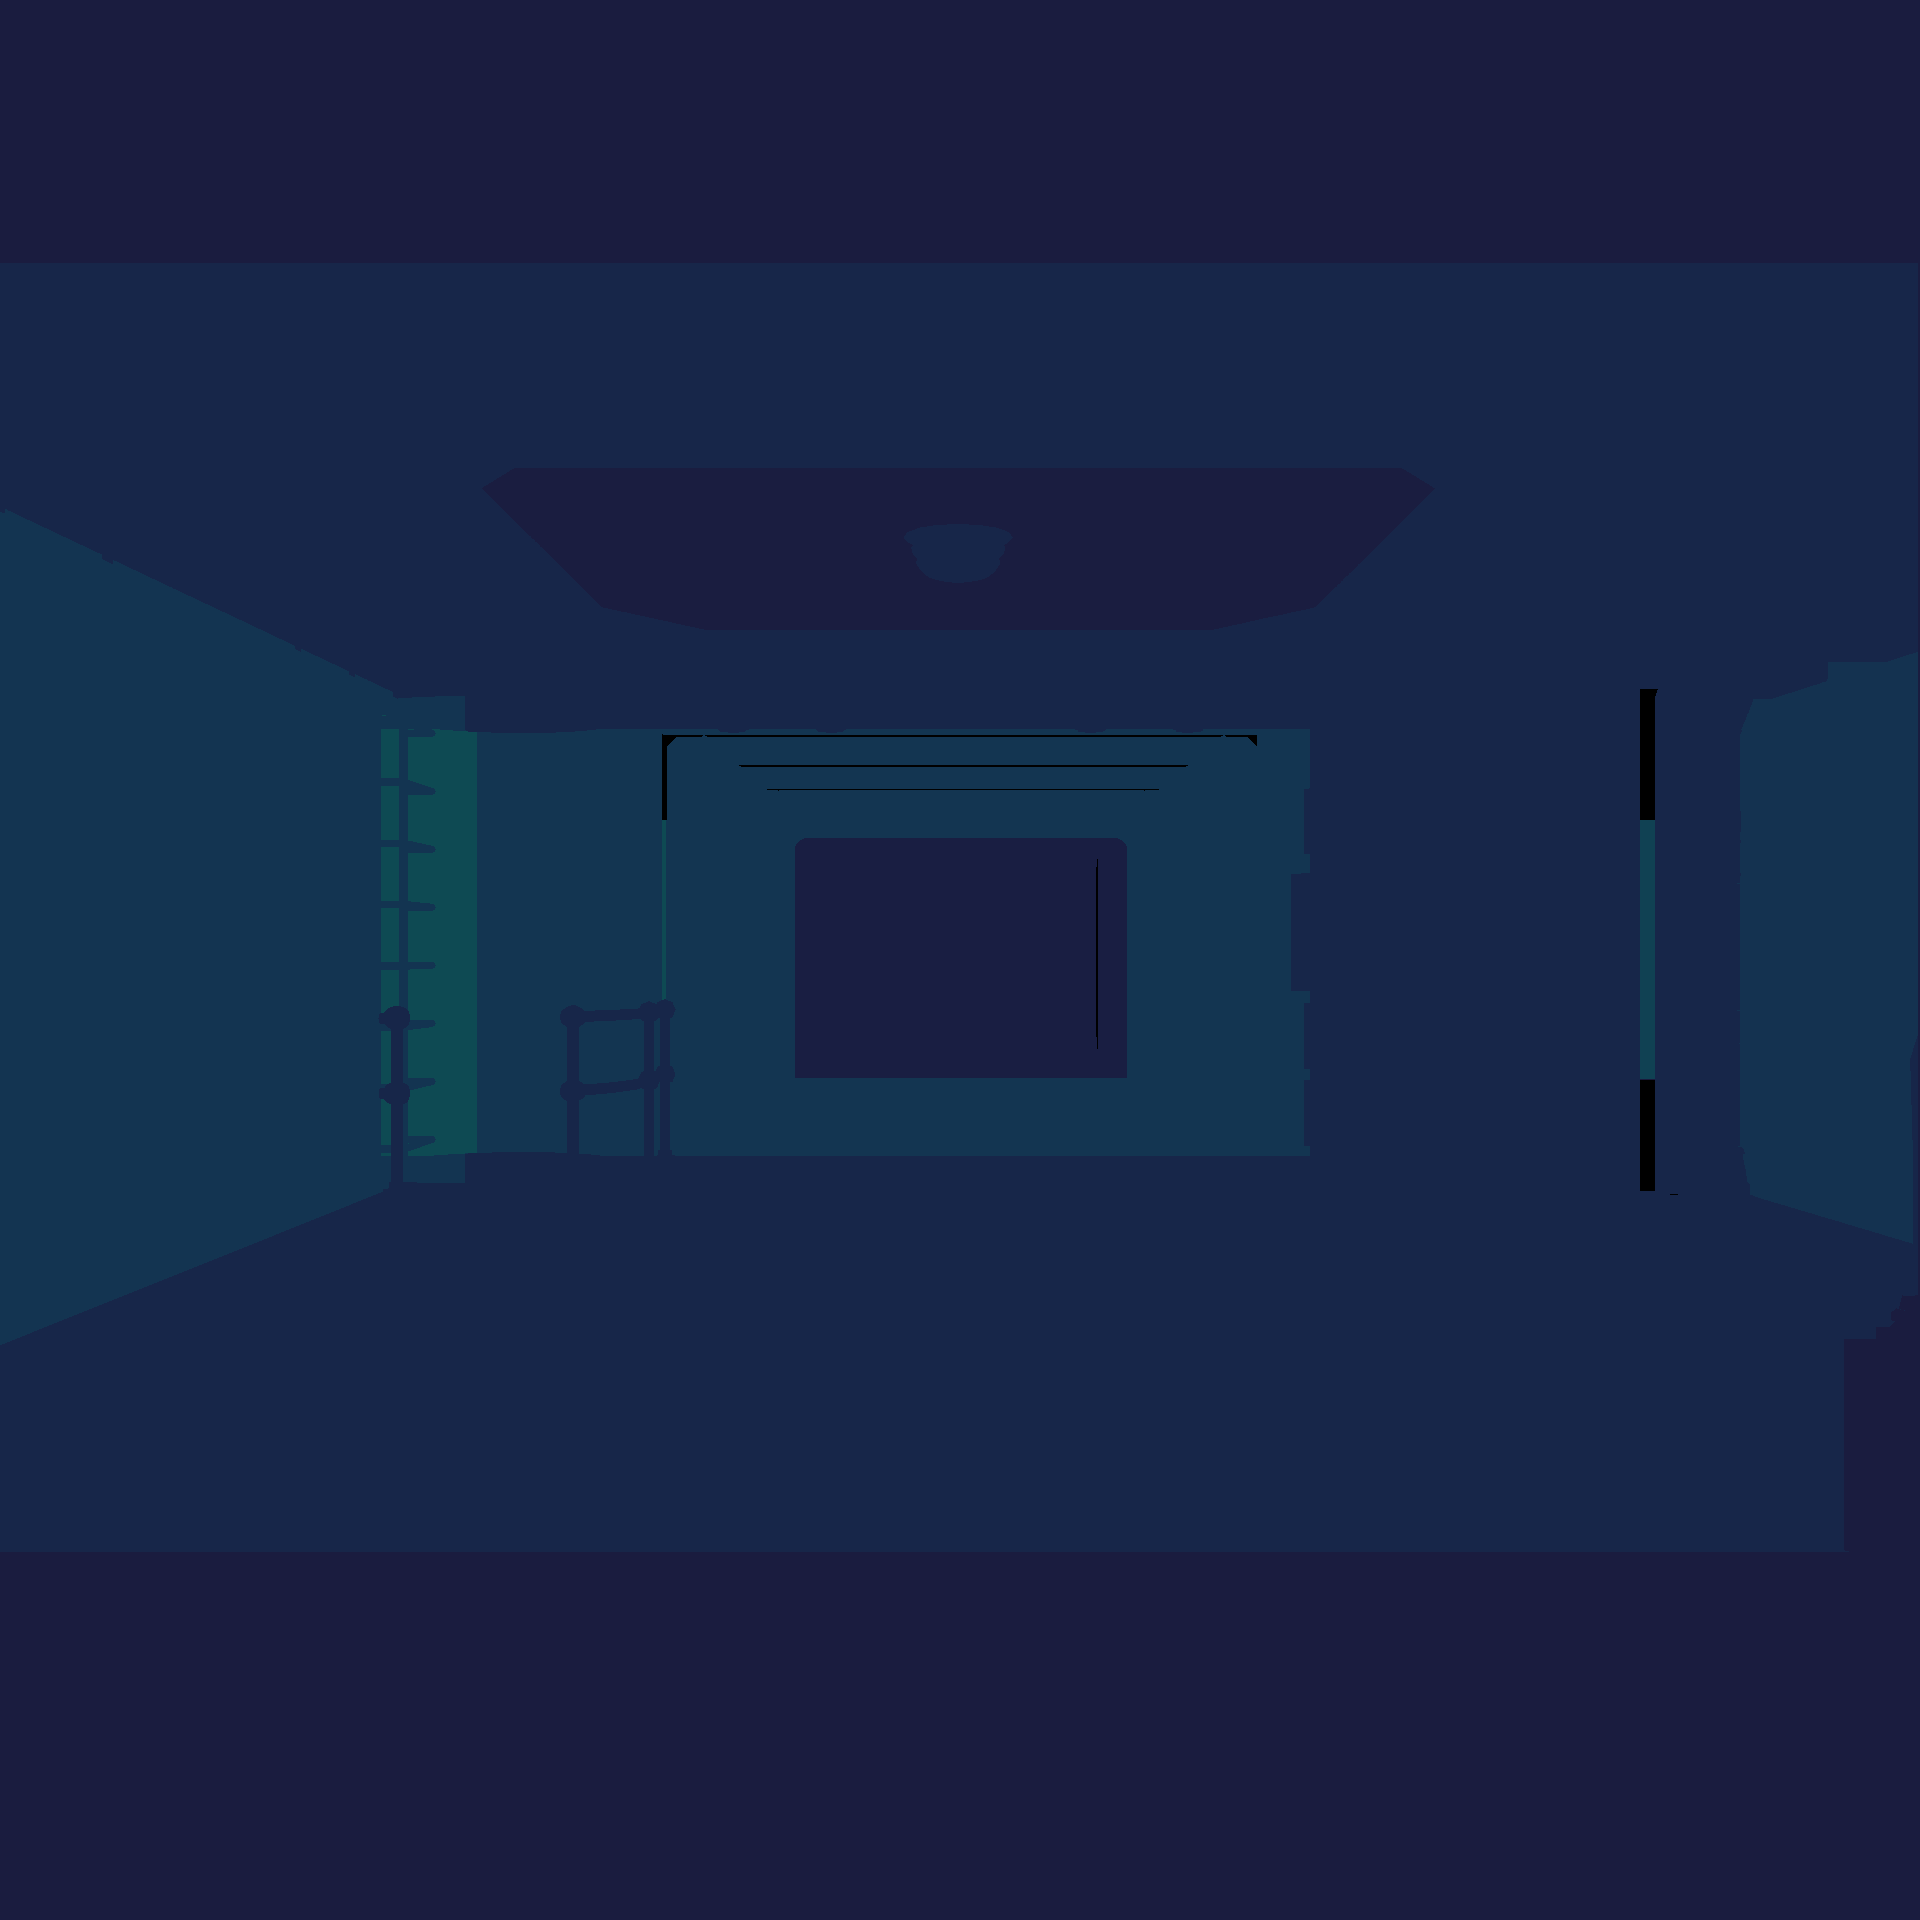
\includegraphics[width=0.275\textwidth]{./img/raw/hs-ns-frames-render/spaceship-indoor/4.png}};

    \node[inner sep=0pt] (img1) at (0.28\textwidth, 0.0\textwidth) {
\includegraphics[width=0.275\textwidth]{./img/raw/hs-ns-frames-render/pipers-alley/0.png}};
    \node[inner sep=0pt] (img1) at (0.28\textwidth,-0.28\textwidth) {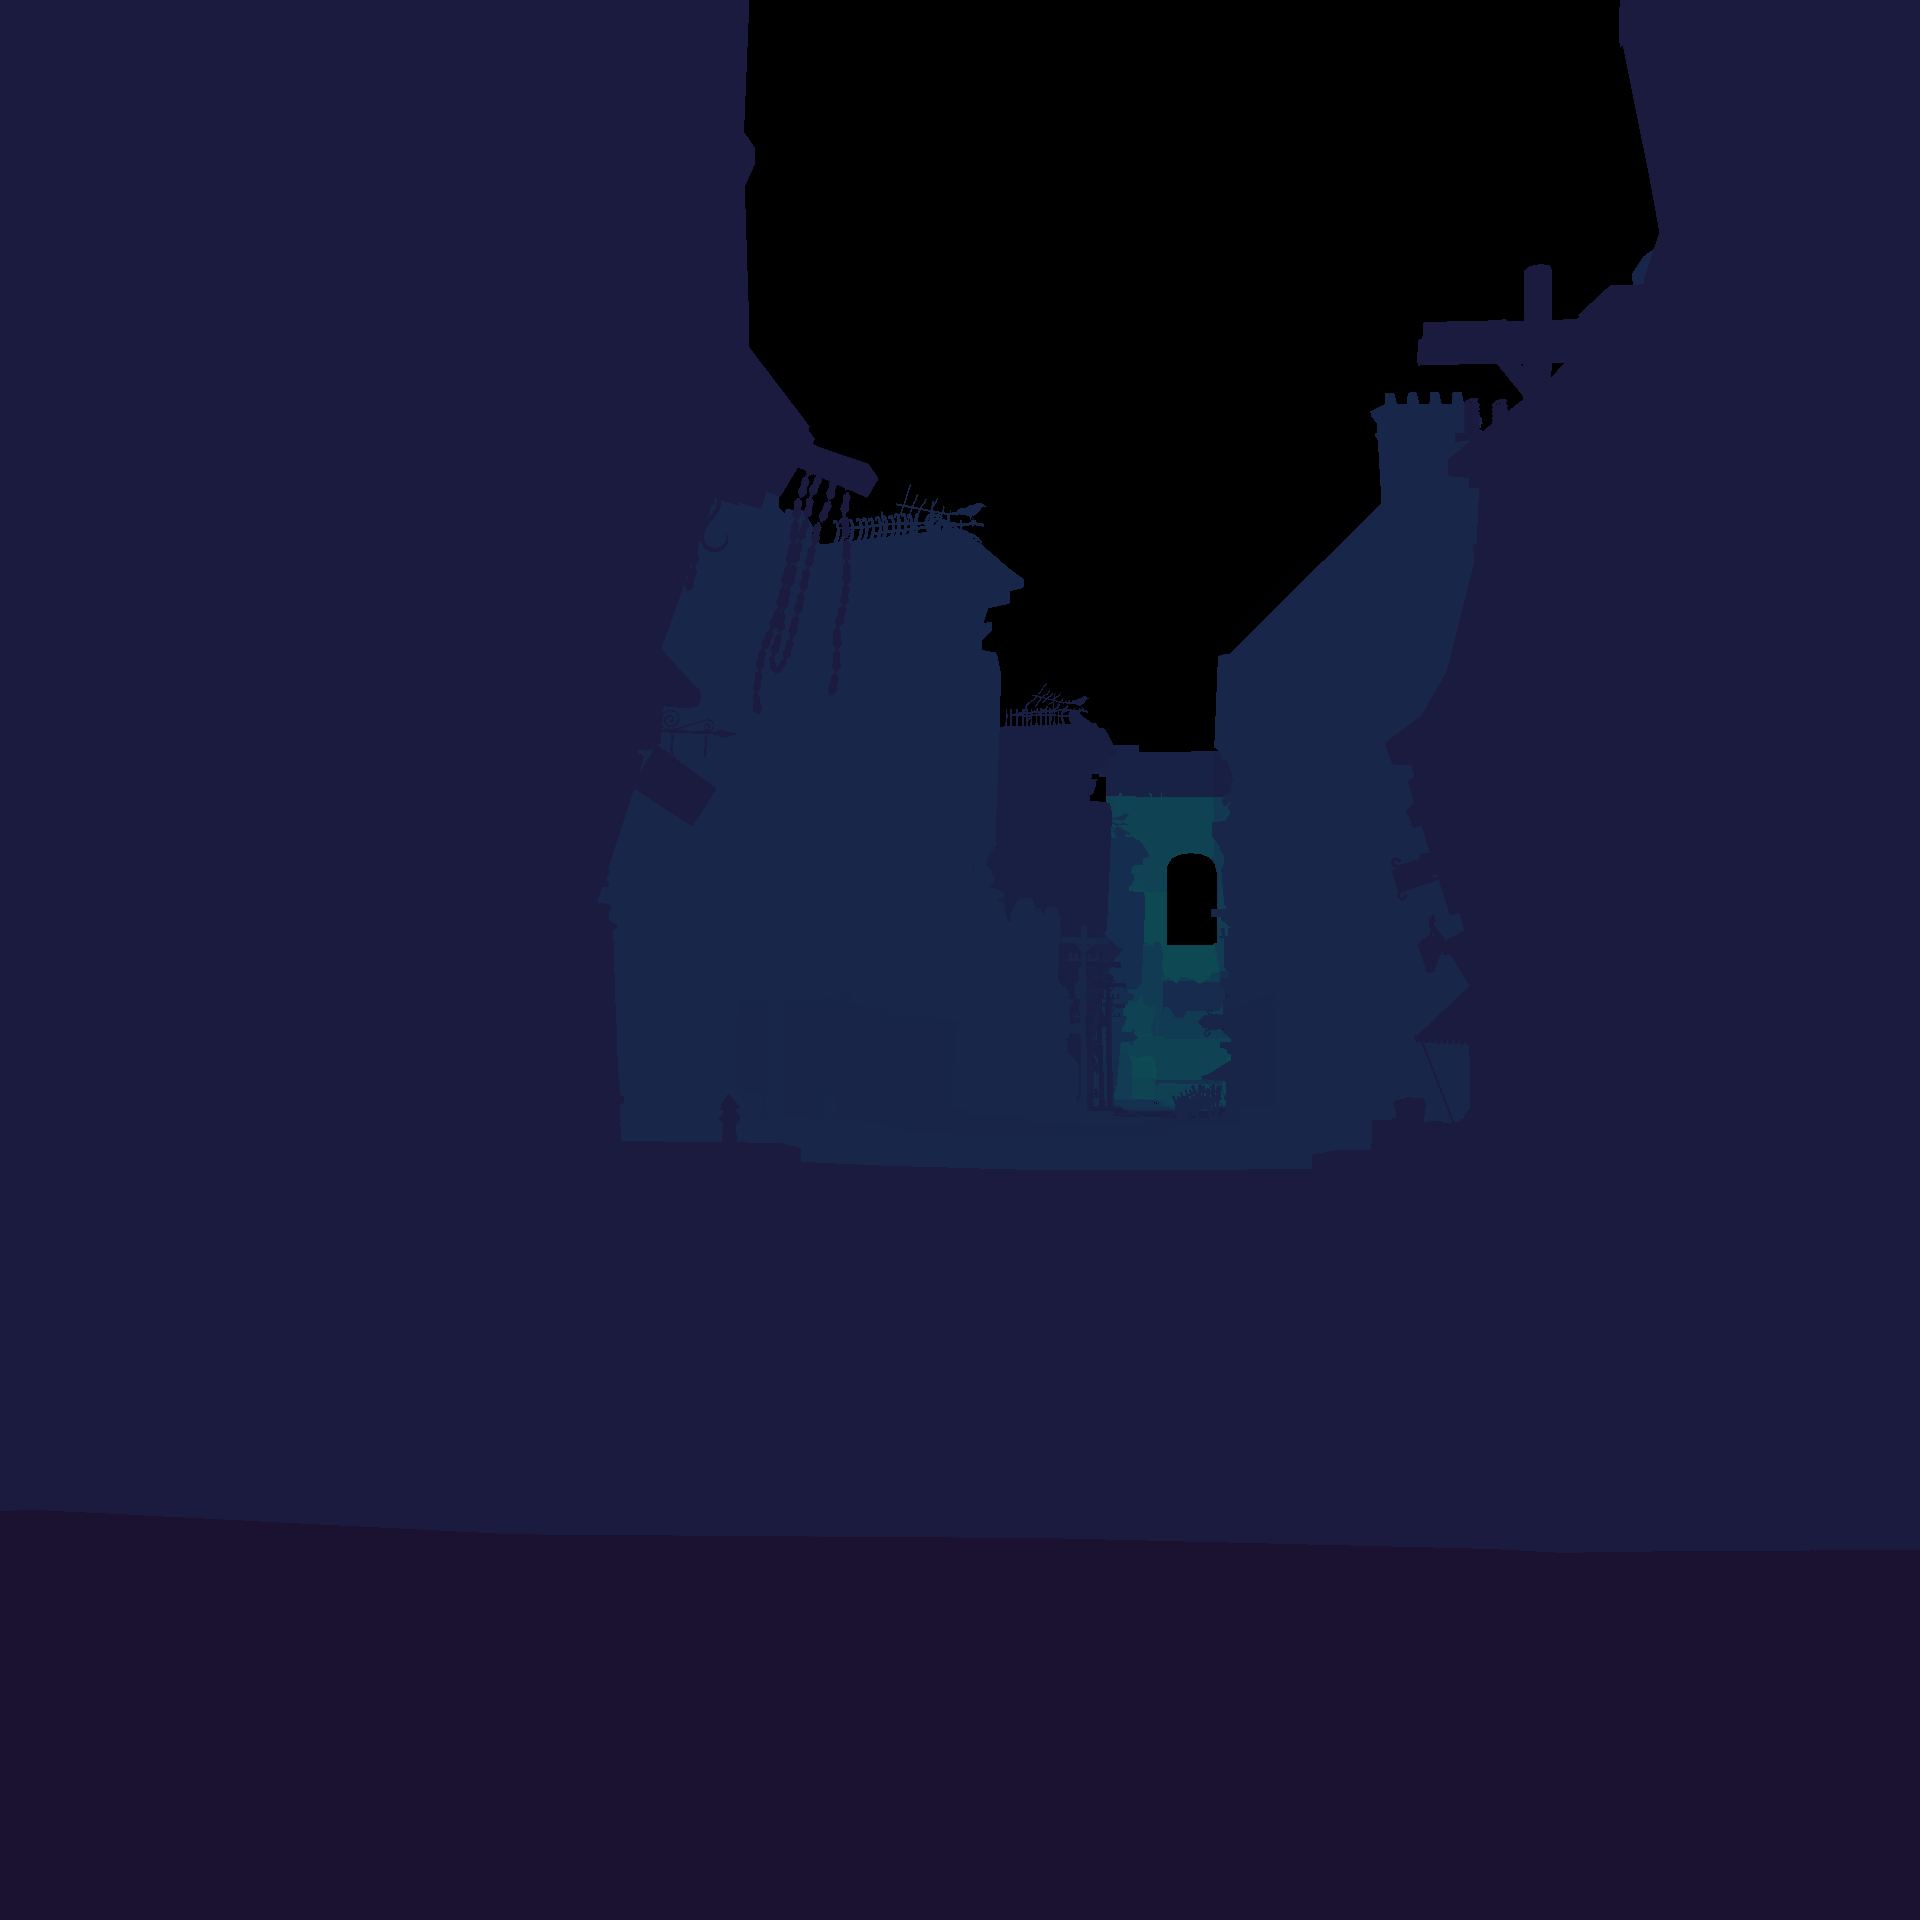
\includegraphics[width=0.275\textwidth]{./img/raw/hs-ns-frames-render/pipers-alley/1.png}};
    \node[inner sep=0pt] (img1) at (0.28\textwidth,-0.56\textwidth) {
\includegraphics[width=0.275\textwidth]{./img/raw/hs-ns-frames-render/pipers-alley/2.png}};
    \node[inner sep=0pt] (img1) at (0.28\textwidth,-0.84\textwidth) {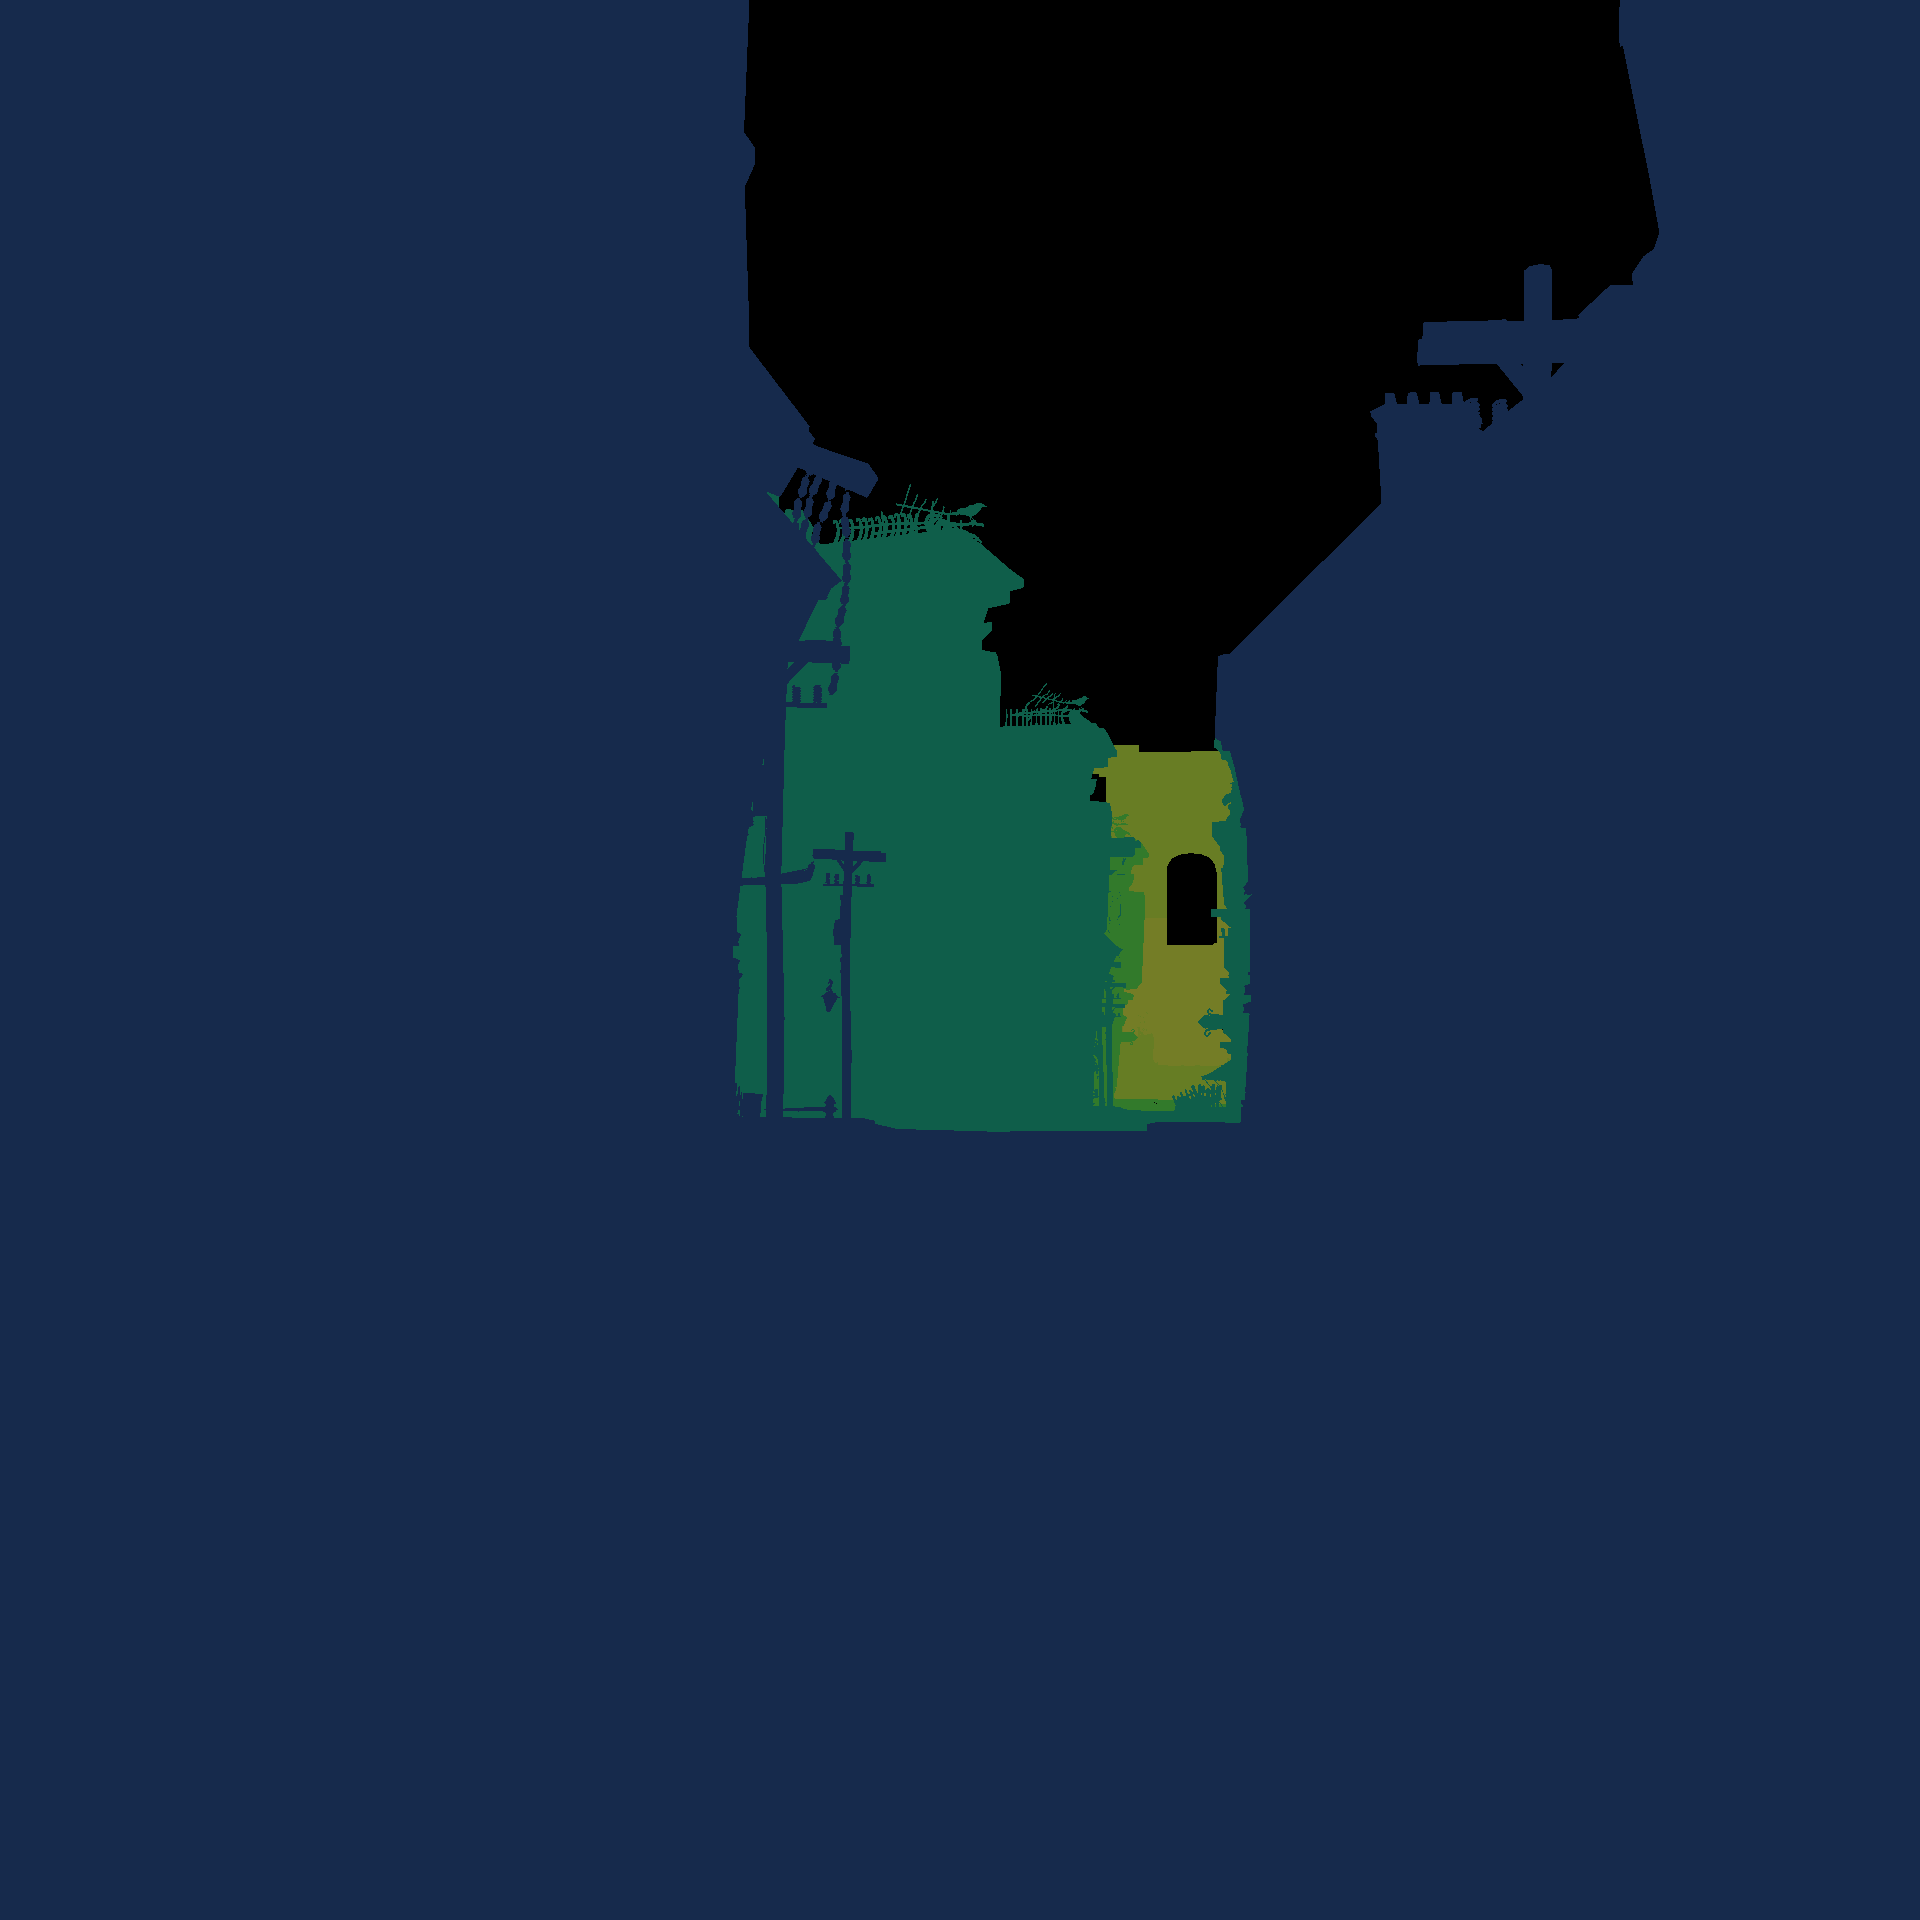
\includegraphics[width=0.275\textwidth]{./img/raw/hs-ns-frames-render/pipers-alley/3.png}};
    \node[inner sep=0pt] (img1) at (0.28\textwidth,-1.12\textwidth) {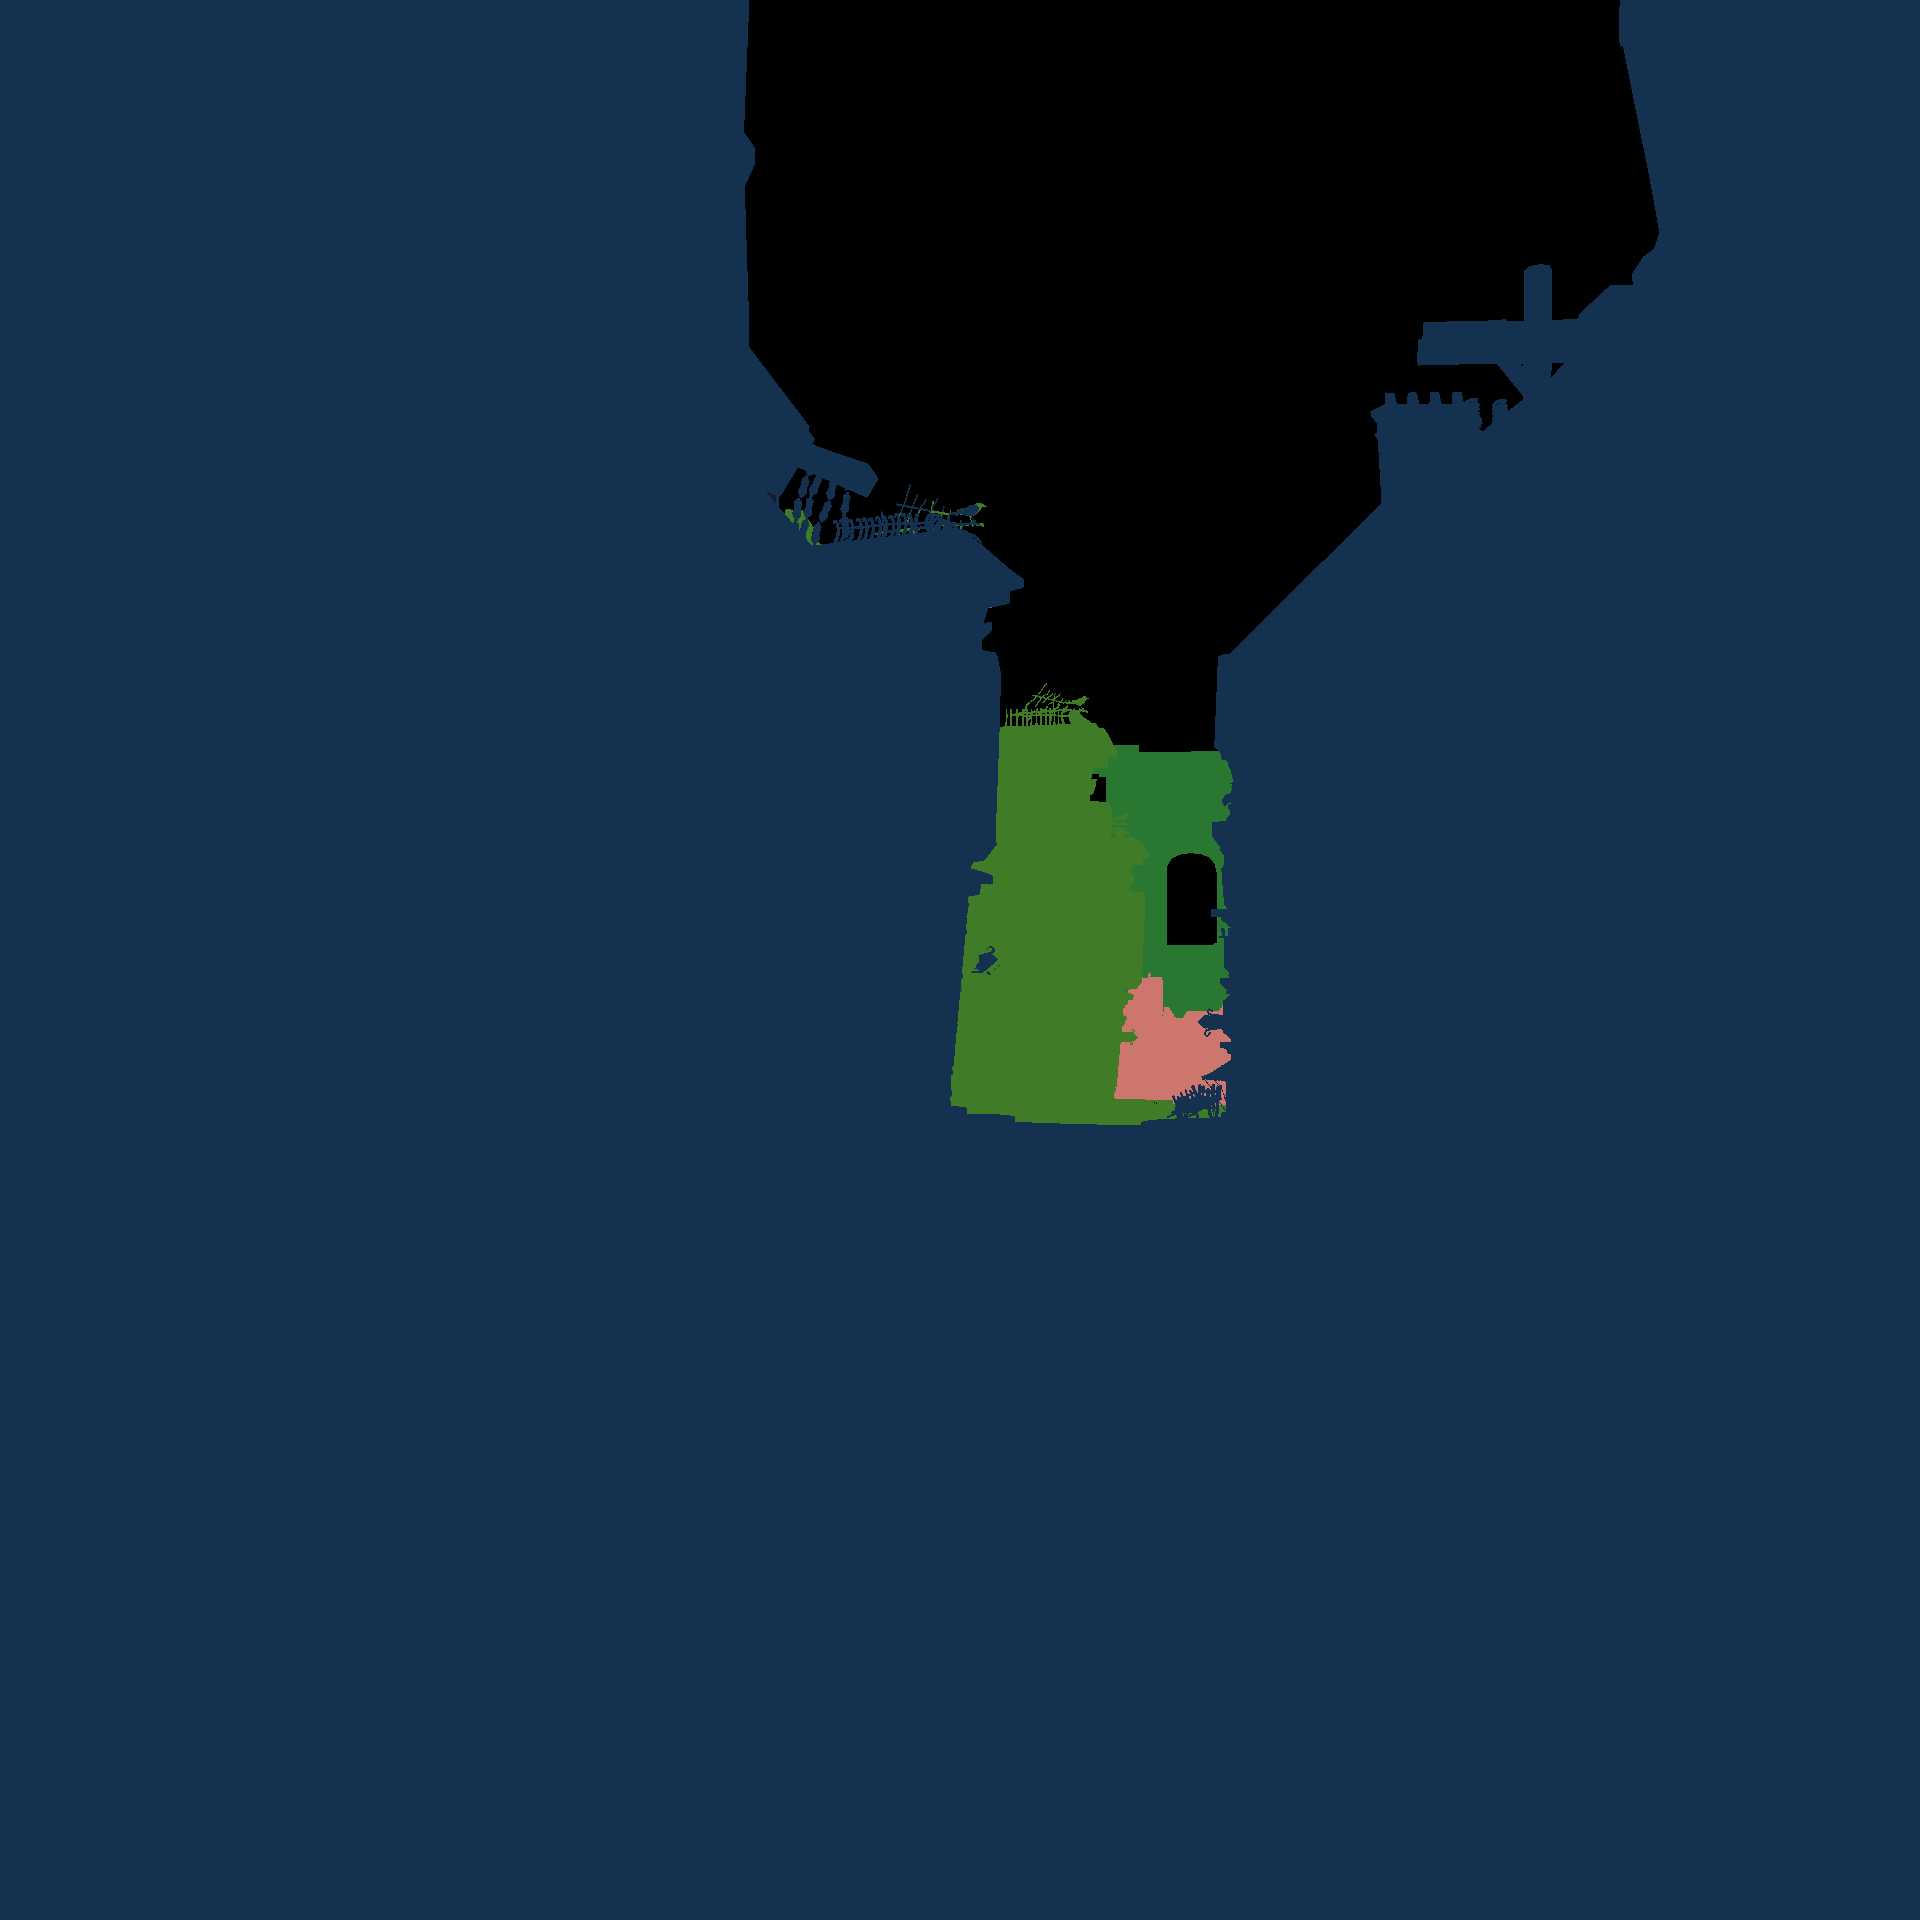
\includegraphics[width=0.275\textwidth]{./img/raw/hs-ns-frames-render/pipers-alley/4.png}};

    \node[inner sep=0pt] (img1) at (0.56\textwidth, 0.0\textwidth) {
\includegraphics[width=0.275\textwidth]{./img/raw/hs-ns-frames-render/ziggurat-city/0.png}};
    \node[inner sep=0pt] (img1) at (0.56\textwidth,-0.28\textwidth) {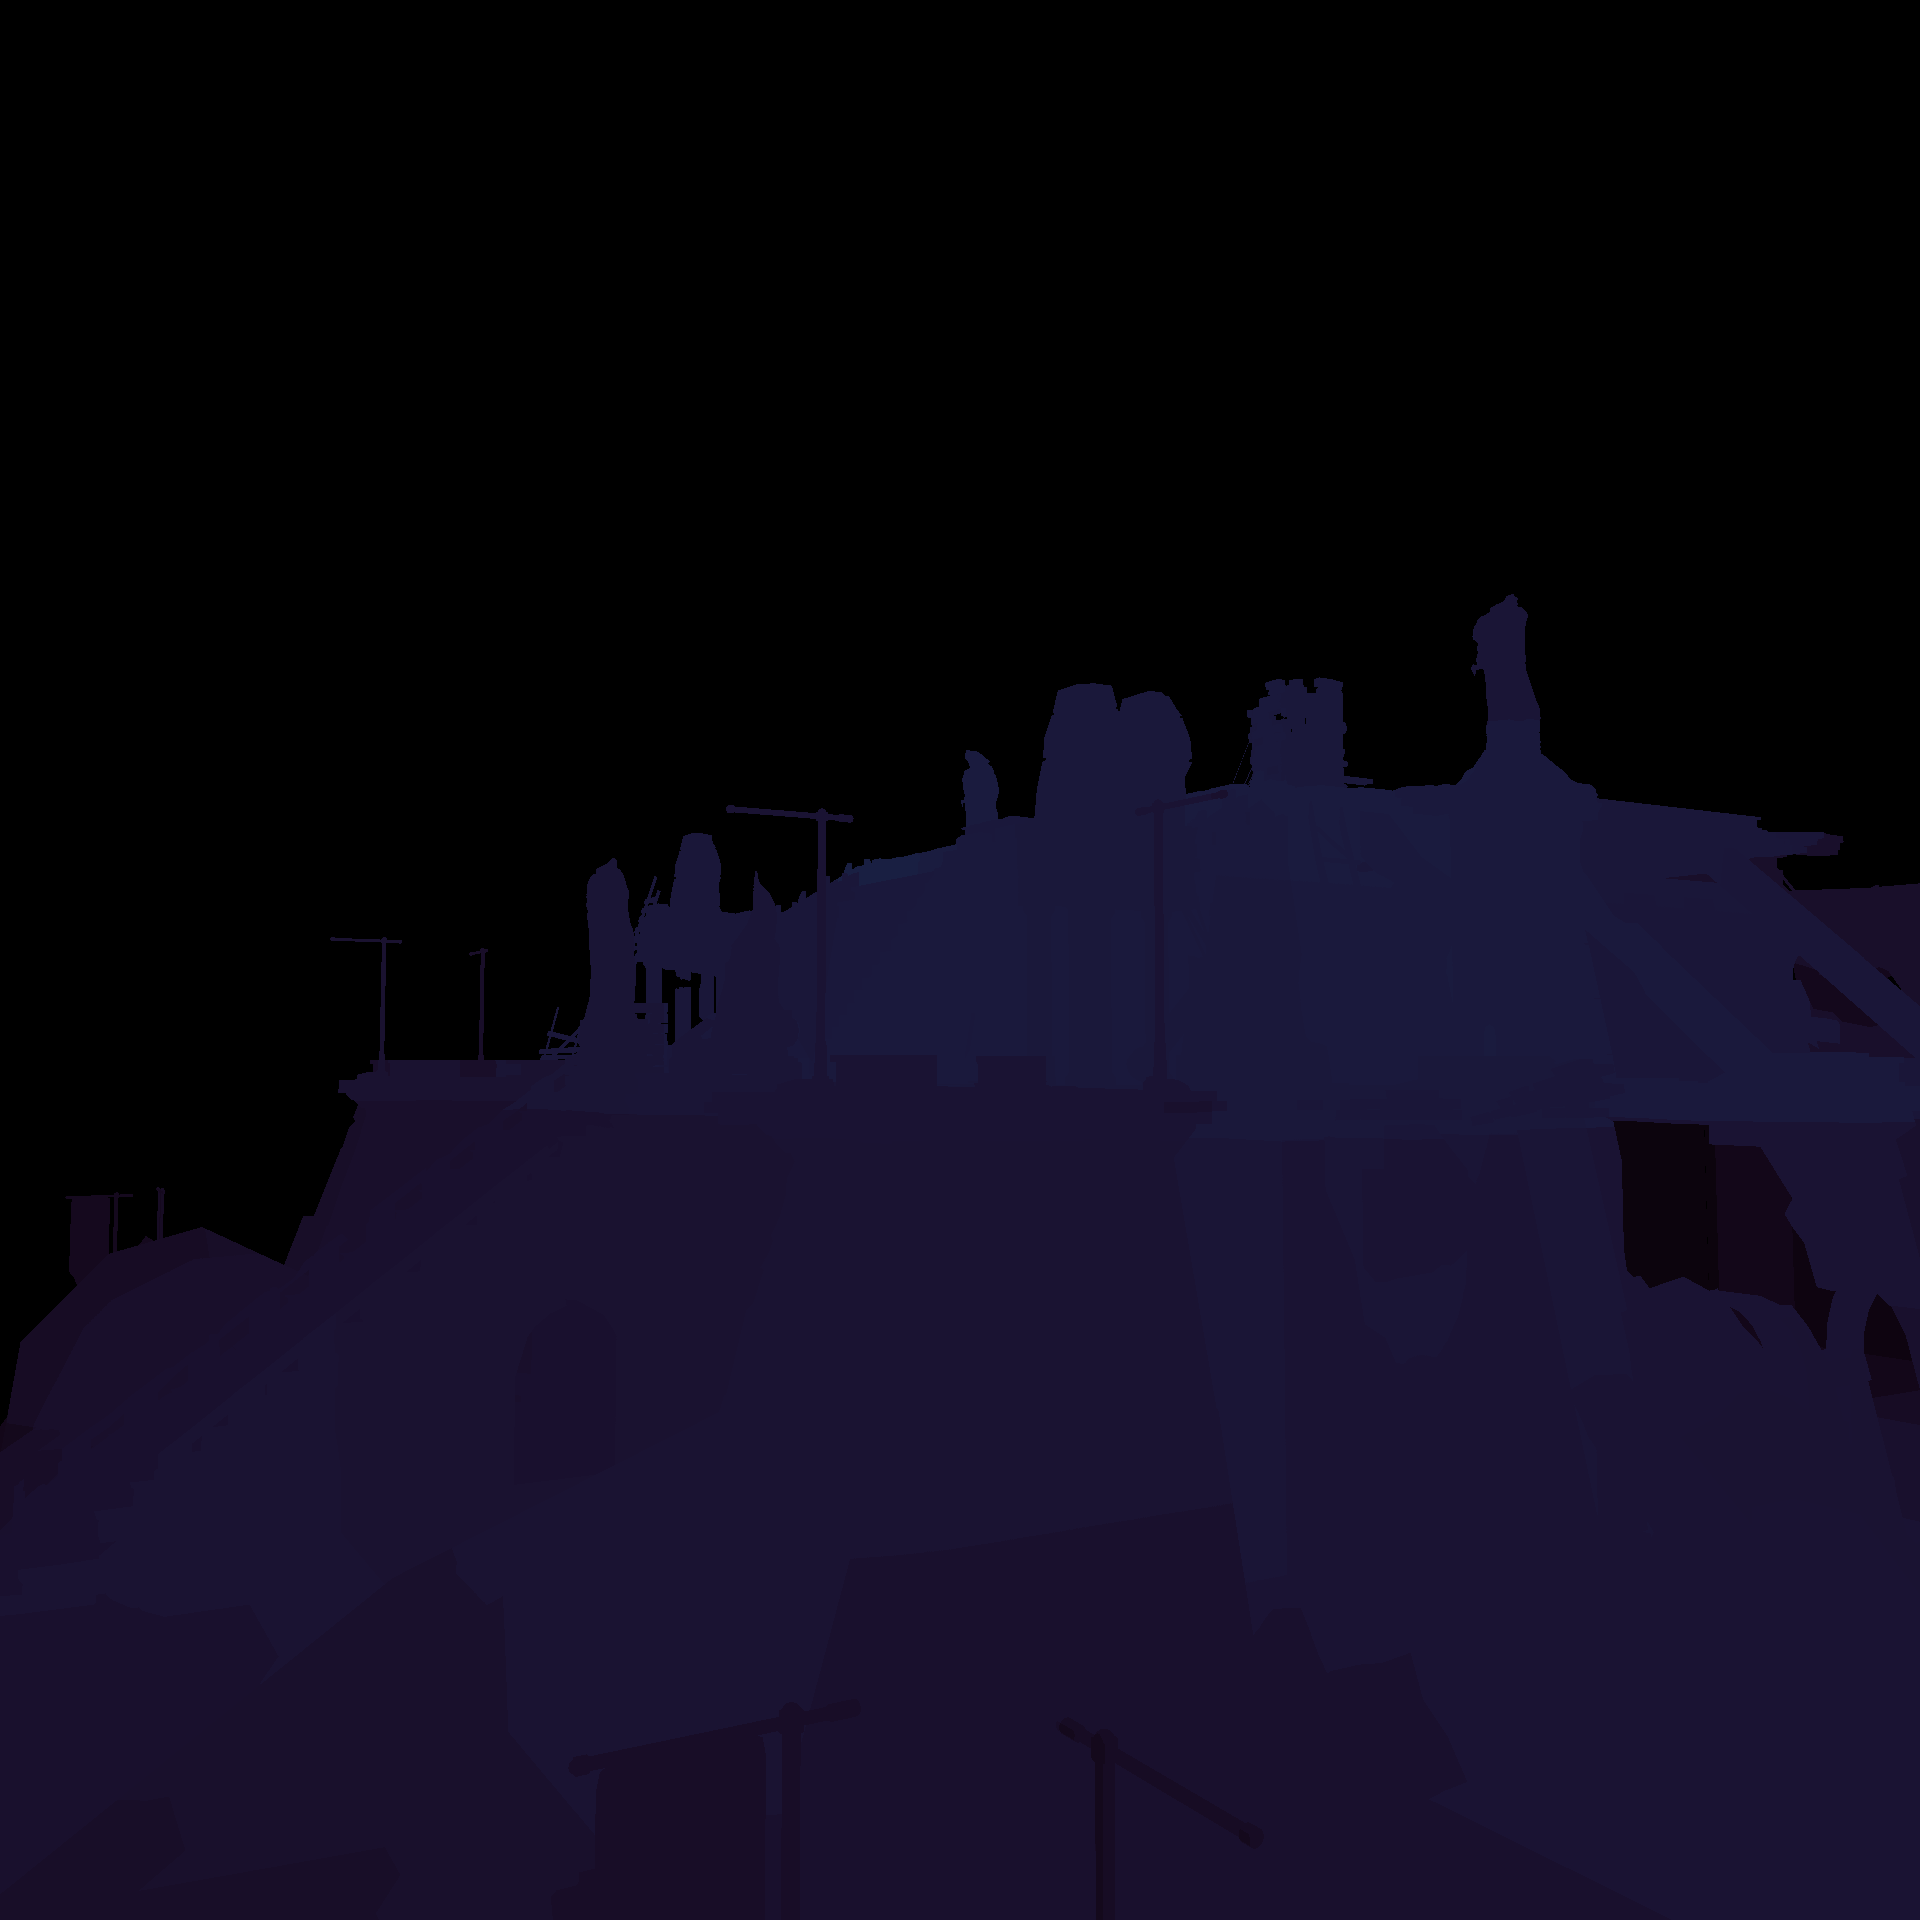
\includegraphics[width=0.275\textwidth]{./img/raw/hs-ns-frames-render/ziggurat-city/1.png}};
    \node[inner sep=0pt] (img1) at (0.56\textwidth,-0.56\textwidth) {
\includegraphics[width=0.275\textwidth]{./img/raw/hs-ns-frames-render/ziggurat-city/2.png}};
    \node[inner sep=0pt] (img1) at (0.56\textwidth,-0.84\textwidth) {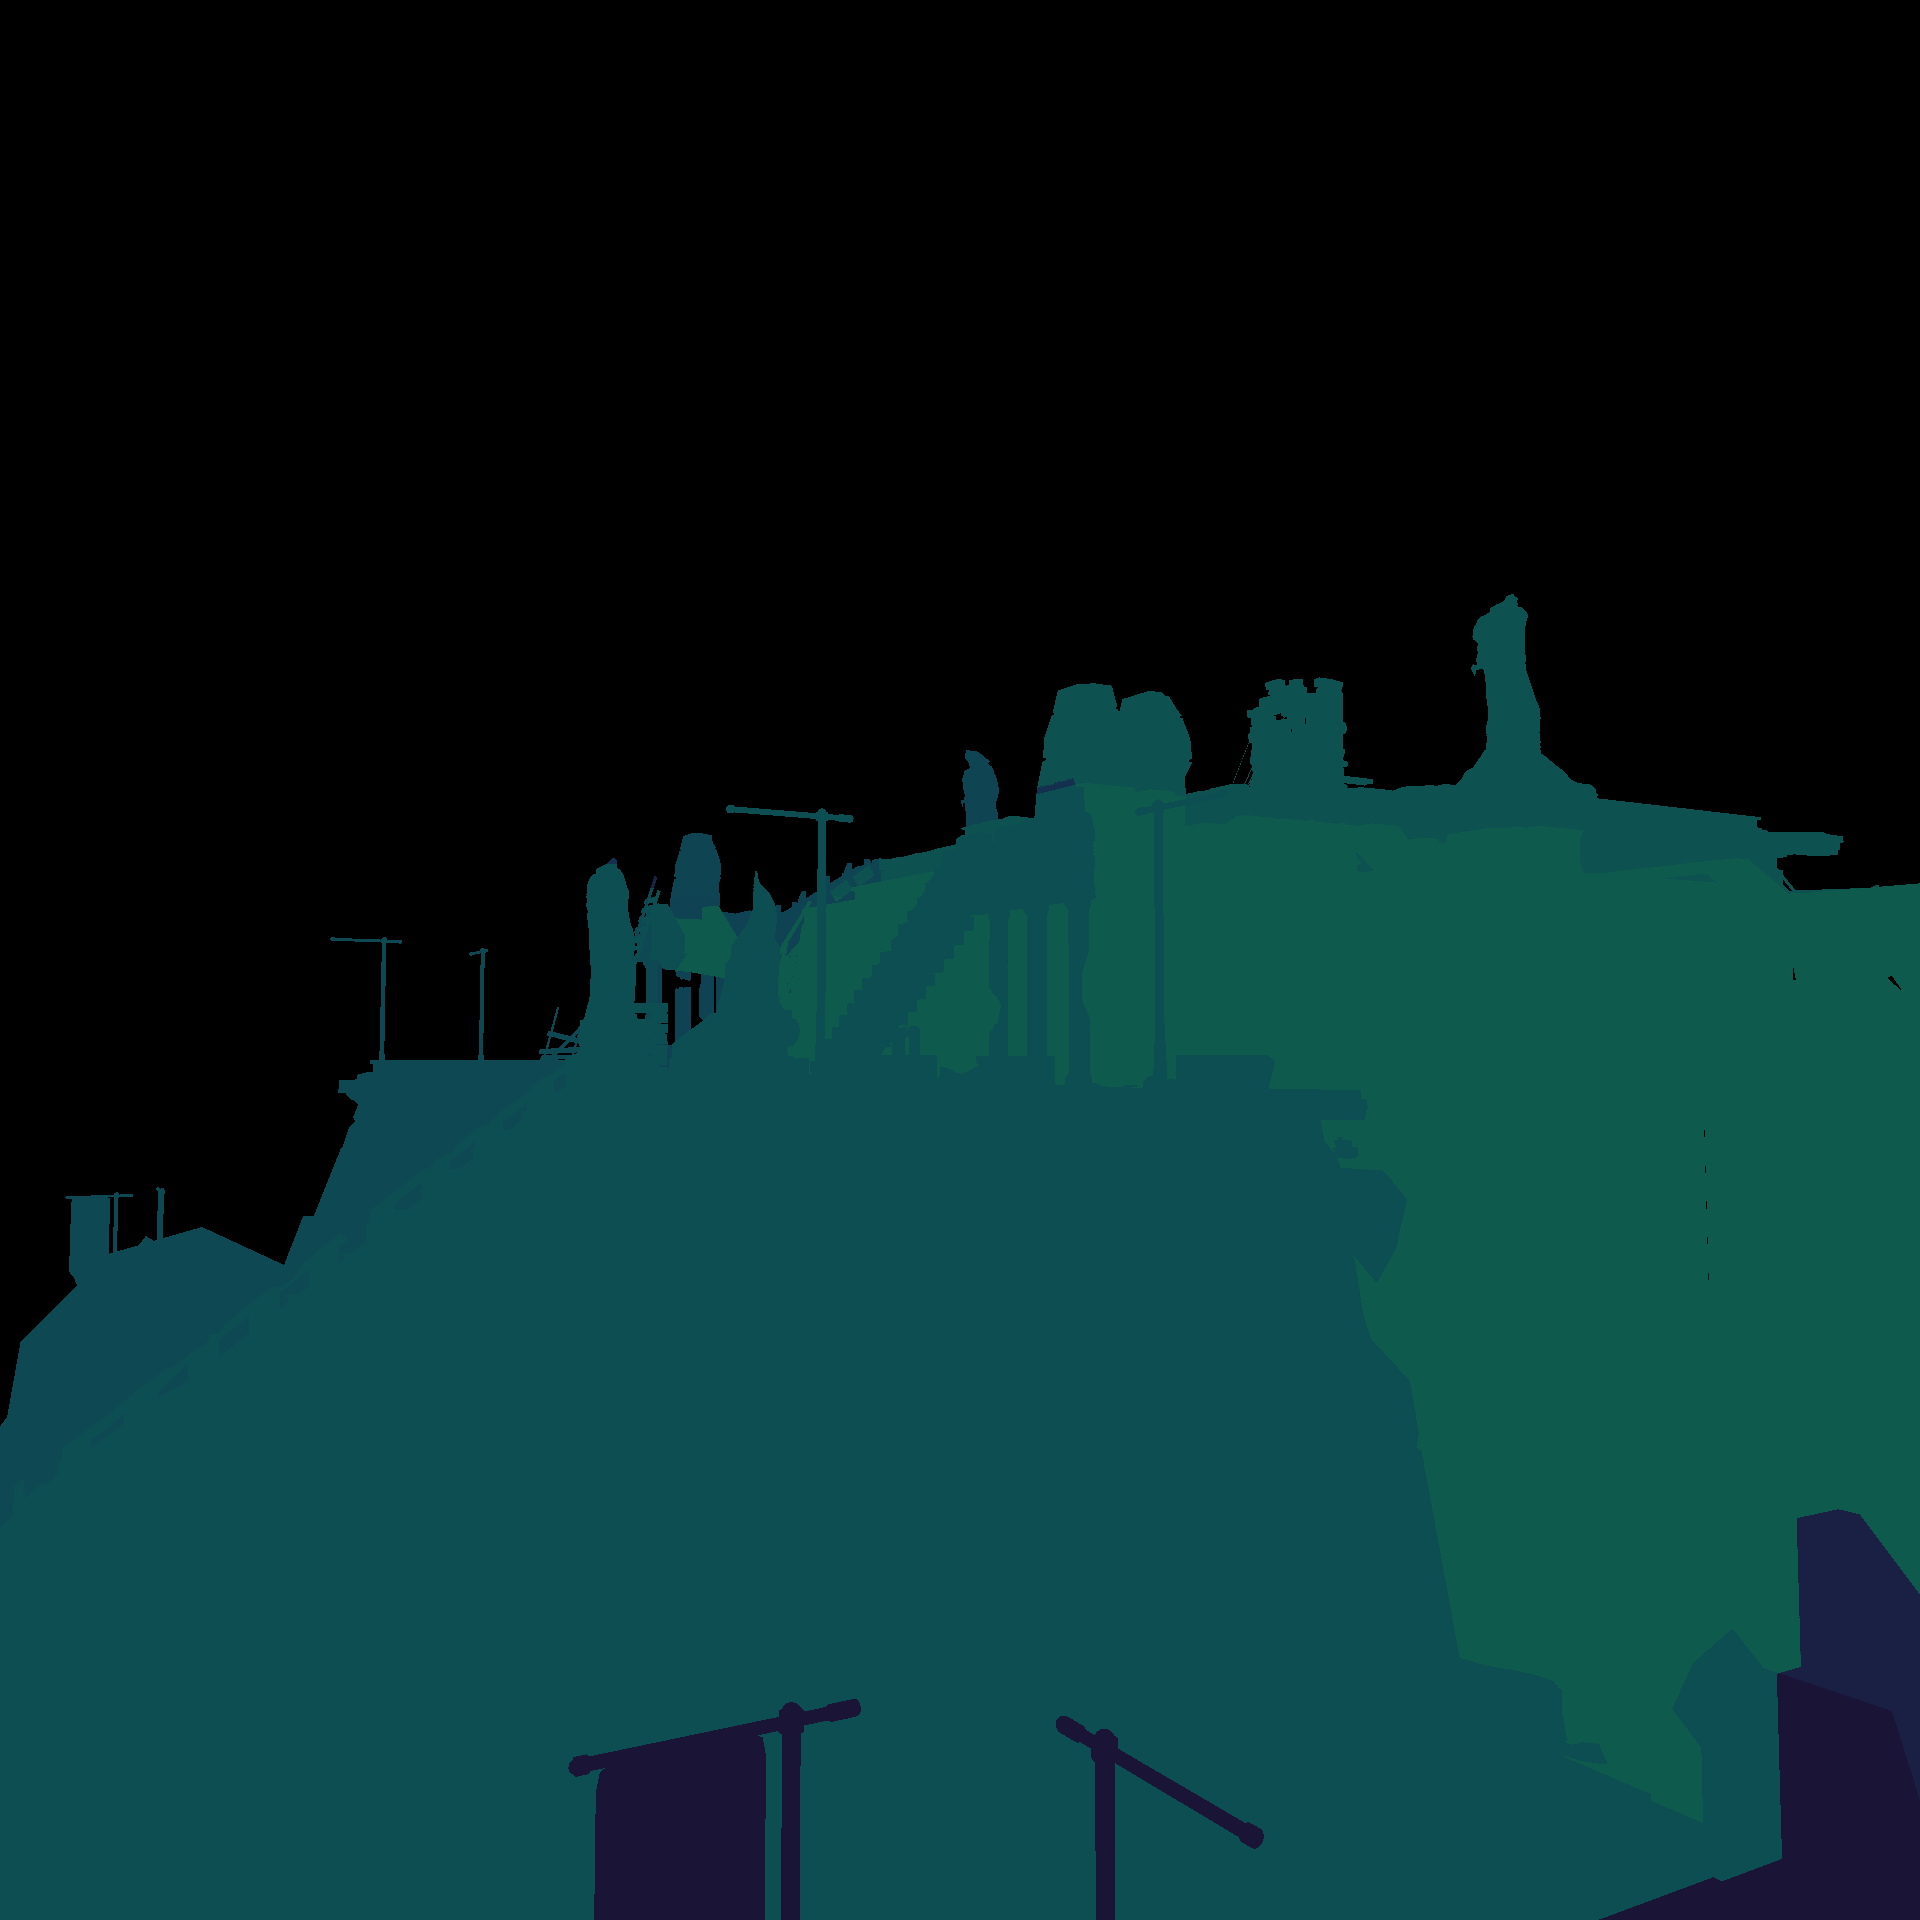
\includegraphics[width=0.275\textwidth]{./img/raw/hs-ns-frames-render/ziggurat-city/3.png}};
    \node[inner sep=0pt] (img1) at (0.56\textwidth,-1.12\textwidth) {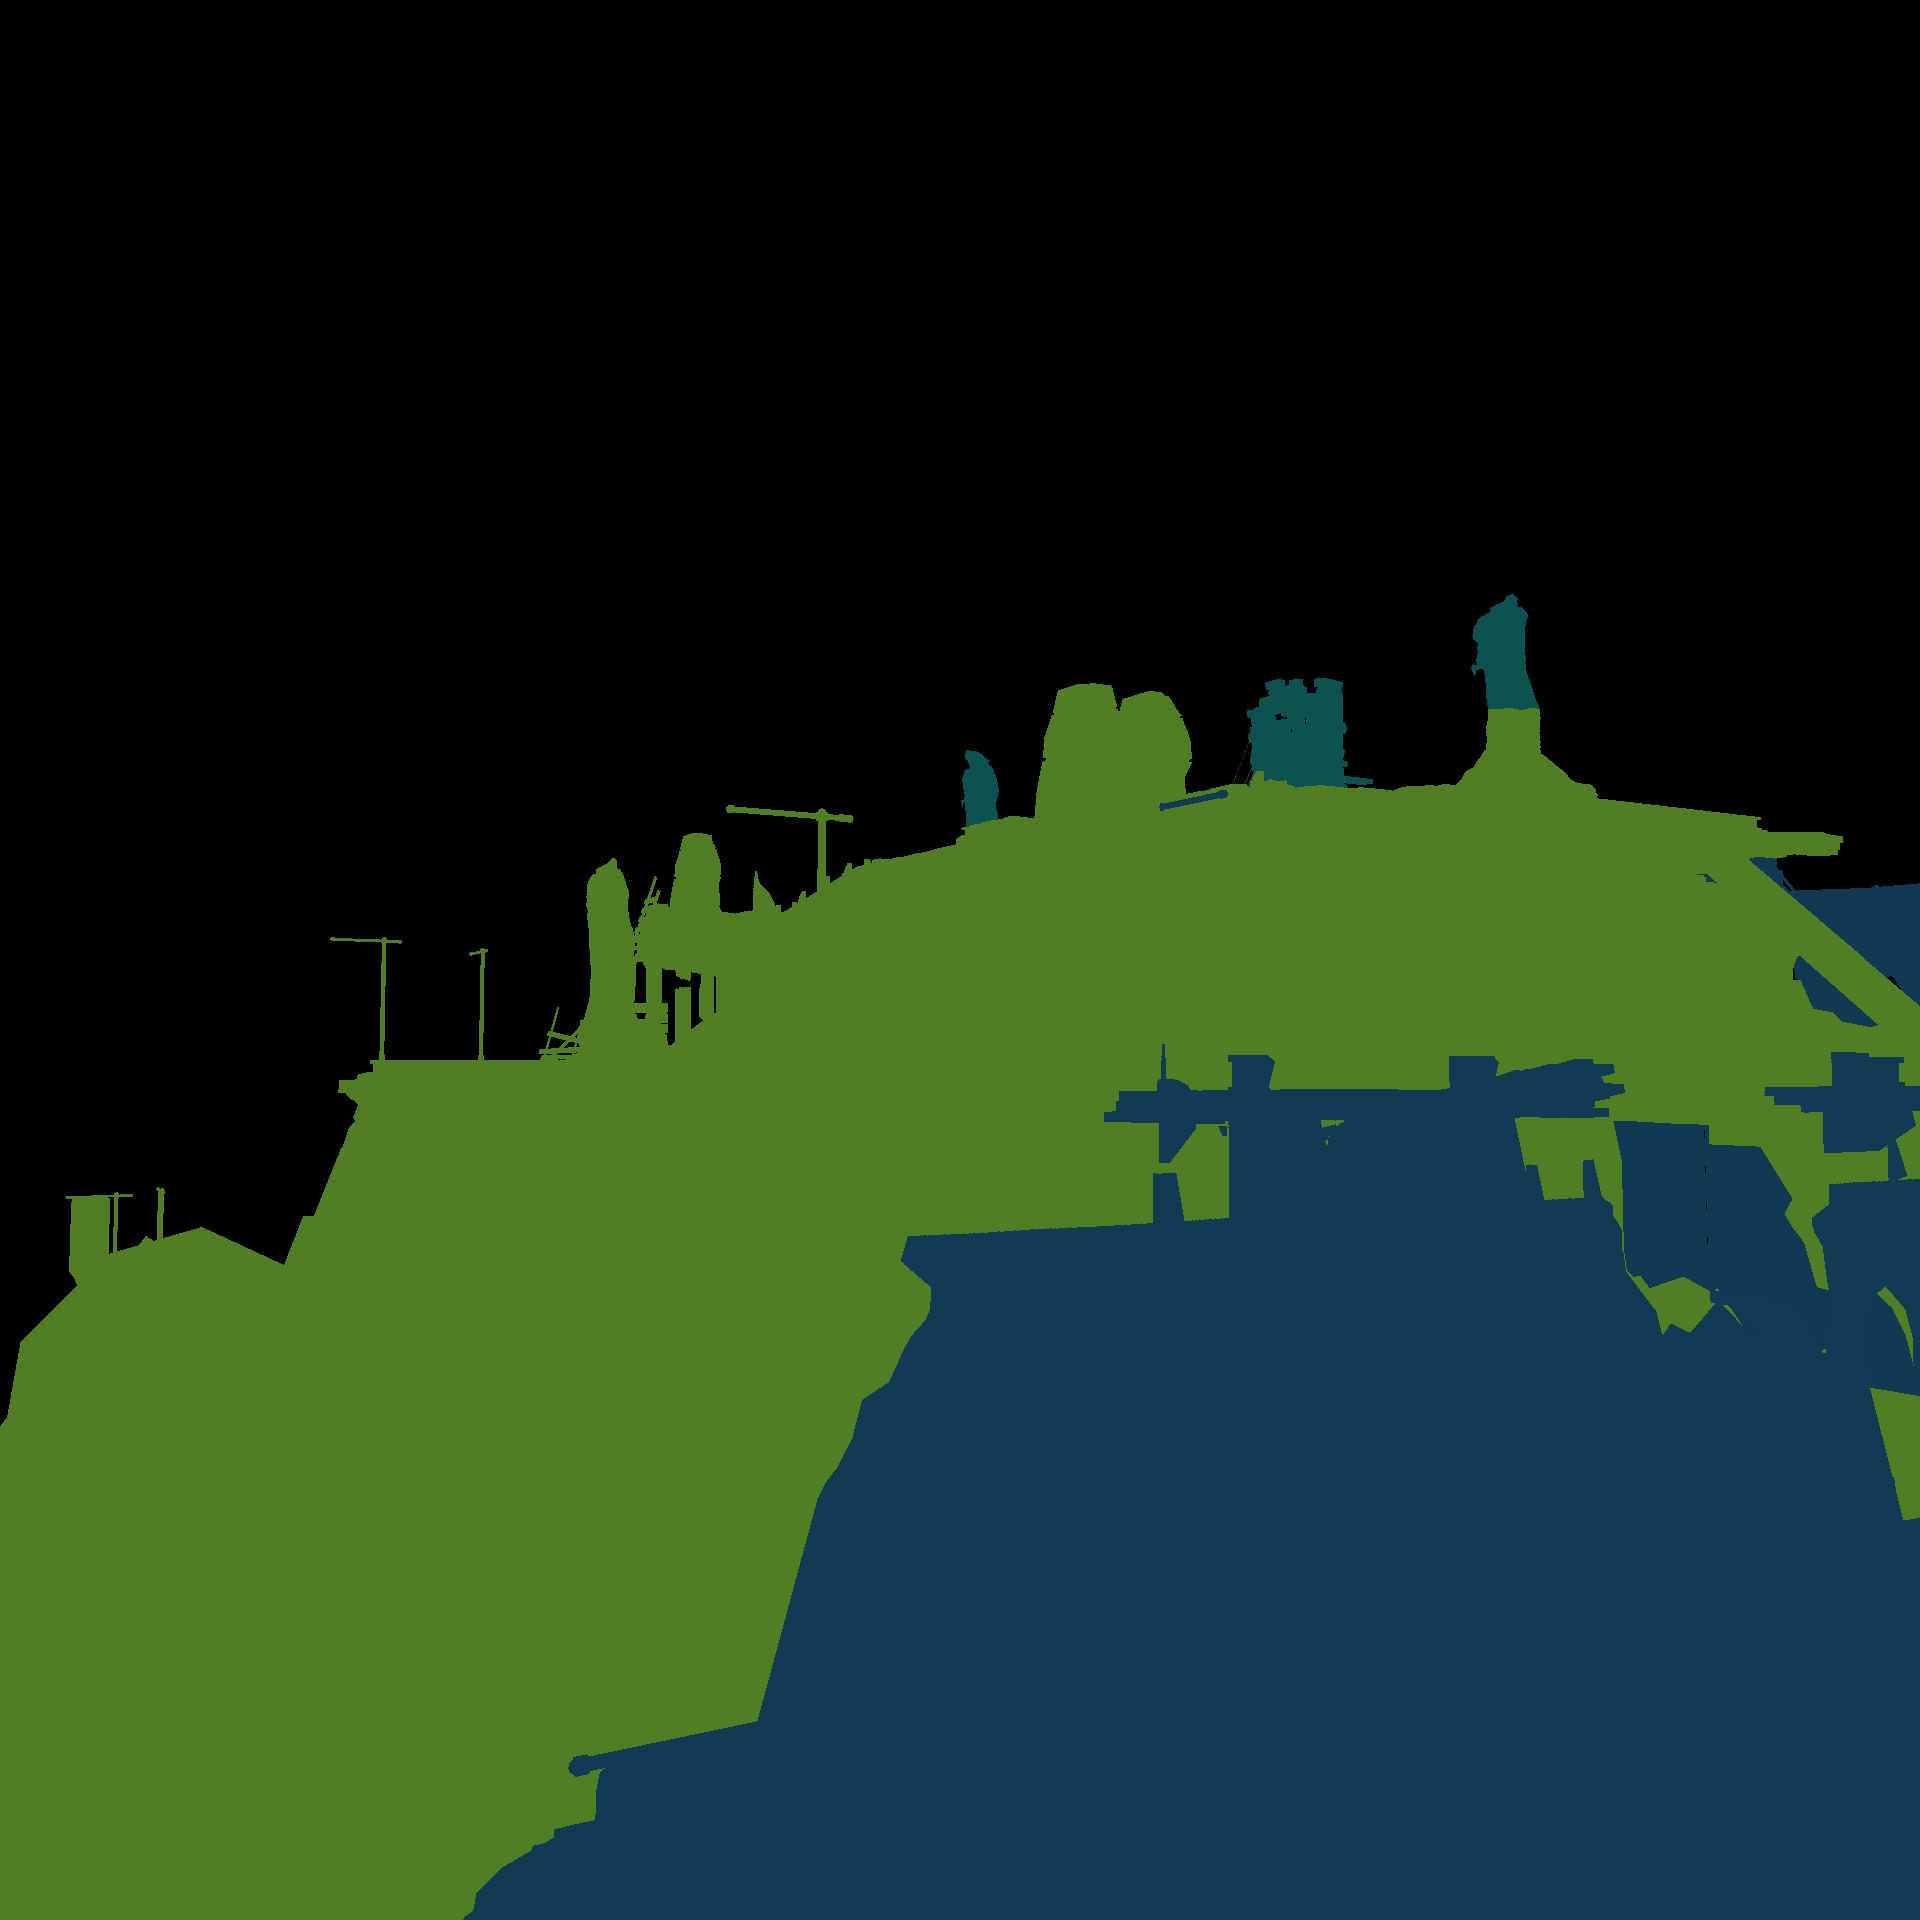
\includegraphics[width=0.275\textwidth]{./img/raw/hs-ns-frames-render/ziggurat-city/4.png}};
  \end{tikzpicture}
  \caption{Visualisatie van het aantal lichtberekeningen bij verschillende knoopgroottes relatief aan het na\"ieve Deferred Shading algoritme.}
  \label{fig:hs-ns-frames-render}
\end{figure}
